\section*{Lecture 3: Parallelization Principles}
We have seen several advantages of parallelism, but there are also some overheads which are not seen in sequential programs like \textbf{communication delay}, \textbf{synchronization} and \textbf{idling}.

\begin{figure}[h]
    \centering
    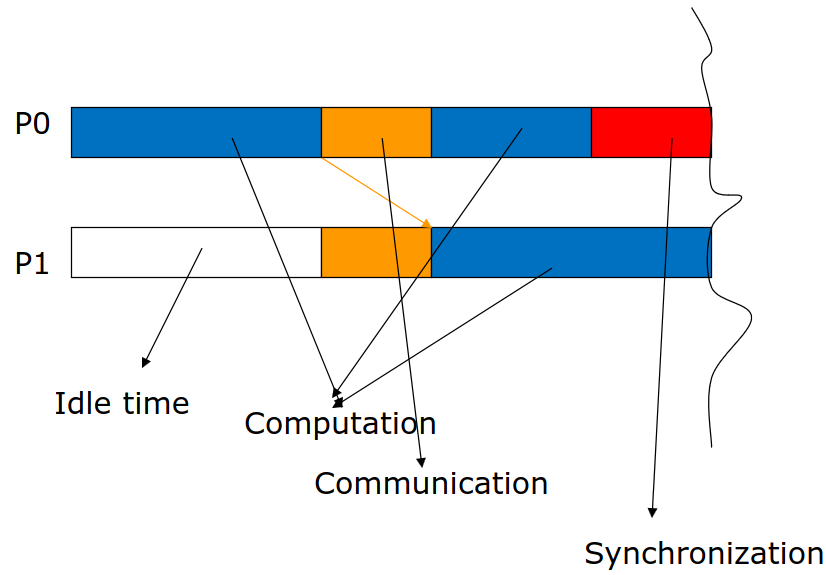
\includegraphics[width=0.5\textwidth]{overheads.png}
    \caption{Overheads}
\end{figure}

\subsection*{Evaluation of Parallel Program}
Let us denote execution time by $T_p$ for parallel program using $p$ processors. \\

1. \textbf{Speedup:} $S(p,n) = T(1,n) / T(p,n)$ where $T(1,n)$ is execution time of sequential program. Usually $S(p,n) \leq p$ as we expect program to get $p$ times faster in idead case but sometimes $S(p,n) > p$ which is called \textbf{superlinear speedup}. Ideally we want $S(p,n) = p$. \\

2. \textbf{Efficiency:} $E(p,n) = S(p,n) / p$. Efficiency is a measure of how well the parallel program is utilizing the resources. Generally $E(p,n) \leq 1$, but in case of superlinear speedup, $E(p,n) > 1$. Ideally we want $E(p,n) = 1$. \\

3. \textbf{Cost:} $C(p,n) = T(p,n) * p$. It is similar to Efficiency but relates the runtime to number of utilized processors. \\

4. \textbf{Scalability:} We want to measure the efficieny of parallel program for variable number of processors. This is called scalability analysis. There are two types of scalability - \textbf{Strong Scalability} and \textbf{Weak Scalability}. In strong scalability, we measure the efficiencies for varying number of processors while keeping indut data size fixed. In weak scalability, we measure efficiency of parallel code by varying both the number of processors and input data size. \\

We will now derive an upper bound on achievable speedup when parallelizing a given sequential program. Let $T_{seq}$ and $T_{par}$ denote the parts whihc cannot benefit from parallelization and can benefit from parallelization respectively. Further assume we can get ideal linear speed up and super linear speedup is also possible. Then we have $T(p,n) \geq T_{seq} + T_{par} / p$. \\

The Speedup is given by \[\Large \boxed{S(p,n) = \frac{T(1,n)}{T(p,n)} \leq \frac{T_{seq} + T_{par}}{T_{seq} + T_{par} / p}}\] 
Instead of using the actual runtimes, now use fraction of the total runtime. Let $f$ be such that $T_{seq} = f * T(1,n)$ and $T_{par} = (1-f) * T(1,n)$. Then we have \[\Large \boxed{S(p,n) \leq \frac{1}{f + \frac{1-f}{p}}}\]

The above equation is known as Amdahl's Law. Now we can see some examples: \\
\begin{enumerate}
    
    \item Suppose 95\% of a rogram’s execution time occurs inside a loop that we want to parallelize. What is the maximum speedup we can expect from a parallel version of our program executed on six processors?
\end{enumerate}

\[\Large \boxed{S(6,n) \leq \frac{1}{0.05 + \frac{0.95}{6}} = 4.8} \]

\begin{enumerate}
    \setcounter{enumi}{1}
    \item 10\% of the program's execution time is spent within sequential code. What is limit to speedup achievable by parallel version ?
\end{enumerate}

Since we are not given how many processors are used, we assume ideal case of unbounded processors.
\[\Large \boxed{ S(\infty,n) \leq \lim_{p \to \infty} \frac{1}{0.1 + \frac{0.9}{p}} = 10} \]

We can see the limitation to Amdahl's Law is that it only applies in situation where problem size is fixed. We will now derive a more general upper bound on speedup. Let $\alpha$ be the scaling function for the sequential part of program and $\beta$ be the scaling function for the parallel part of program. Both $\alpha$ and $\beta$ are w.r.t to complexity of problem size. \\
This means $T_{seq}$ grows as $\alpha * T(1,n)$ as problem size grows and $T_{par}$ grows as $\beta * T(1,n)$ as problem size grows. \\

\[ T_{\alpha \beta} (1,n) = \alpha * T_{seq} + \beta * T_{par} = \alpha * f * T(1,n) + \beta * (1-f) * T(1,n) \]
\[ T_{\alpha \beta} (p,n) = \alpha * T_{seq} + \frac{\beta * T_{par}}{p} = \alpha * f * T(1,n) + \frac{\beta * (1-f) * T(1,n)}{p} \]

Then we have \[\Large \boxed{S_{\alpha \beta}(p,n) \leq \frac{\alpha * f + \beta * (1-f)}{\alpha * f + \frac{\beta * (1-f)}{p}}}\]

Let $\gamma = \frac{\beta}{\alpha}$, then we have \[\Large \boxed{S_{\gamma}(p,n) \leq \frac{f + \gamma * (1-f)}{f + \frac{\gamma * (1-f)}{p}}}\]

Now depending on the value of $\gamma$, we can have different upper bounds on speedup. 
\begin{enumerate}
    \item Amdahl's Law: $\gamma = 1$ which means $\alpha = \beta$
    \item Gustafson's Law: $\gamma = p$ which means $\alpha=1$ and $\beta=p$. This means parallel part of program grows linearly in $p$ as problem size grows. In this case the formula becomes \[\Large \boxed{S(p,n) \leq f + (1-f) * p}\]
    
    This law can also be thought as by knowing f , we can use it to predict the
    theoretically achievable speedup using multiple processors when parallelizable part scales linearly with the problem size while the serial part remains constant
\end{enumerate}

let us discuss some examples: \\
\begin{enumerate}
    \item Suppose we have a parallel program that is 15\% serial and 85\% linearly parallelizable for a given problem size. Assume that the (absolute) serial time does not grow as the problem size is scaled.\\
    
    (i) How much speedup can we achieve if we use 50 processors without scaling the problem - $S_{\gamma=1}(50,n)$
    (ii) Suppose we scale up the problem size by a factor of 100. How much speedup could we achieve with 50 processors - $S_{\gamma=100}(50,n)$
\end{enumerate}

\subsection*{Roofline Performance Model}
This gives a bound on the performance of an application on a particular architecture and it also helps to categorize the code's performance as memory bound or performance bound. It depends on three parameters - Peak Performance of the machine $P_{peak} \;\; (FLOP/s)$, Memory Bandwidth $B_{peak} \;\; (Bytes/s)$ and Computational Intensity $I_{op} \;\; (FLOP/Byte)$. \\

\subsection*{Questions / Doubts}
1. Discuss this Roofline Model again with Professor and work out some examples. \\